\documentclass[fleqn, a4paper, 12pt, twoside]{article}

\newcounter{recitationcount} %creates a new counter for recitation numbers (must be executed before exsheets is loaded)
\newcommand\recitation{\refstepcounter{recitationcount}}

\usepackage[counter-within = recitationcount]{exsheets}
\usepackage{amsmath, amssymb, amsthm} %standard AMS packages
\usepackage{mathtools}
\usepackage{marginnote} %marginnotes
\usepackage{gensymb} %miscellaneous symbols
\usepackage{commath} %differential symbols
\usepackage{xcolor} %colours
\usepackage{cancel} %cancelling terms
%\usepackage{siunitx} %formatting units
\usepackage{tikz, pgfplots} %diagrams
	\usetikzlibrary{calc, hobby, patterns, intersections}
\usepackage{graphicx} %inserting graphics
\usepackage{hyperref} %hyperlinks
\usepackage{datetime} %date and time
\usepackage{ulem} %underline for \emph{}
\usepackage{xfrac} %inline fractions
\usepackage{enumerate} %numbered lists
\usepackage{float} %inserting floats
\usepackage[siunitx, americanvoltages, americancurrents]{circuitikz} %circuit diagrams

\newcommand\numberthis{\addtocounter{equation}{1}\tag{\theequation}} %adds numbers to specific equations in non-numbered list of equations

\newcommand{\AxisRotator}[1][rotate=0]{
	\tikz [x=0.25cm,y=0.60cm,line width=.2ex,-stealth,#1] \draw (0,0) arc (-150:150:1 and 1);%
} %rotation symbols on axes

\theoremstyle{definition}
\newtheorem{example}{Example}
\newtheorem{definition}{Definition}

\theoremstyle{theorem}
\newtheorem{theorem}{Theorem}

\newcommand{\curl}{\mathrm{curl\,}}

\makeatletter
\@addtoreset{section}{part} %resets section numbers in new part
\makeatother

\newcommand\blfootnote[1]{%
	\begingroup
	\renewcommand\thefootnote{}\footnote{#1}%
	\addtocounter{footnote}{-1}%
	\endgroup
}

\RenewQuSolPair{question}[name=Recitation \therecitationcount\ -- Exercise]{solution}[name=Recitation \therecitationcount\ -- Solution]

\SetupExSheets{solution/print = true, totoc = true} %prints all solutions by default

%opening
\title{Introduction to Electrical Engineering}
\author{Aakash Jog}
\date{2014-15}

\begin{document}

\maketitle
%\setlength{\mathindent}{0pt}

\blfootnote
{	
	\begin{figure}[H]
		\includegraphics[height = 12pt]{cc.eps}
		\includegraphics[height = 12pt]{by.eps}
		\includegraphics[height = 12pt]{nc.eps}
		\includegraphics[height = 12pt]{sa.eps}
	\end{figure}
	This work is licensed under the Creative Commons Attribution-NonCommercial-ShareAlike 4.0 International License. To view a copy of this license, visit \url{http://creativecommons.org/licenses/by-nc-sa/4.0/}.
} %CC-BY-NC-SA licencse

\tableofcontents

 \newpage
%\part{General Information}

\section{Instructor Information}

\textbf{Naftali Landsberg}\\
~\\
Telephone: \href{tel:+97236406422}{+972 3-640-6422}\\
Mobile: \href{tel:+972544293212}{+972 54-429-3212}\\
E-mail: \href{mailto:naftali.landsberg@gmail.com}{naftali.landsberg@gmail.com}\\

\newpage
\part{}

\section{}

\recitation

\begin{question}
	\begin{figure}[H]
		\begin{circuitikz}
			\draw 
				(0,0) to [battery1 = 32 \si{\volt}, i = $I_1$] 							(0,5) 
						to [R = 2 \si{\kilo\ohm}, i = $I_1$, v = $\Delta V_1$] (5,5) 
						to [R = 4 \si{\kilo\ohm}, i = $I_3$, v = $\Delta V_3$] (10,5);
			\draw 
				(10,0) to [battery1 = 20 \si{\volt}, i< = $I_3$] (10,5);
			\draw 
				(5,5) to [R = 8 \si{\kilo\ohm}, i = $I_2$, v = $\Delta V_2$] (5,0);
			\draw 
				(0,0) to (5,0) to (10,0);
		\end{circuitikz}
	\end{figure}
\end{question}

\begin{solution}
	By KCL for the upper junction,
	\begin{equation*}
		I_1 - I_2 - I_3 = 0
	\end{equation*}
	By KCL for the lower junction,
	\begin{equation*}
		-I_1 + I_2 + I_3 = 0
	\end{equation*}
	By KVL for left loop,
	\begin{equation*}
		-32 + \Delta V_1 + \Delta V_2 = 0
	\end{equation*}
	By KVL for right loop,
	\begin{equation*}
		-20 - \Delta V_2 + \Delta V_3 = 0
	\end{equation*}
	By KVL for the larger loop,
	\begin{equation*}
		32 - \Delta V_1 - \Delta V_2 - 20 = 0
	\end{equation*}
\end{solution}

\begin{question}
	\begin{figure}[H]
		\begin{circuitikz}
			\coordinate (1) at (0,5);
			\coordinate (2) at (2,5);
			\coordinate (3) at (7,5);
			\coordinate (4) at (12,5);
			
			\coordinate (5) at (0,0);
			\coordinate (6) at (2,0);
			\coordinate (7) at (7,0);
			\coordinate (8) at (12,0);
			
			\draw 
				(1) to [short, i = 3 \si{\ampere}] (2)
				(2) to [R = 3 \si{\ohm}, i = $i_4$] (3)
				(3) to [short, i< = $i_3$] (4)
				(5) to [short, i< = 3 \si{\ampere}] (6)
				(6) to [short, i< = $i_5$] (7)
				(7) to [battery1 = 10 \si{\volt}, i = $i_3$] (8)
				(5) to [current source = 3 \si{\ampere}] (1)
				(6) to [R = 2 \si{\ohm}, i< = $i_1$] (2)
				(7) to [R = 4 \si{\ohm}, i< = $i_2$] (3)
				(8) to [R = 5 \si{\ohm}, i< = $i_3$] (4);
		\end{circuitikz}
	\end{figure}
\end{question}

\begin{solution}
	By KCL at $2$,
	\begin{equation*}
		3 - i_1 - i_4 = 0
	\end{equation*}
	By KCL at $3$,
	\begin{equation*}
		i_4 + i+3 + i_2 = 0
	\end{equation*}
	By KCL at $6$,
	\begin{equation*}
		-i_3 - i_2 - i_5 = 0
	\end{equation*}
	By KCL at $7$,
	\begin{equation*}
		i_5 + i_1 - 3 = 0
	\end{equation*}
	By KVL in loop A,
	\begin{equation*}
		2 i_1 - V_x = 0
	\end{equation*}
	By KVL in loop B,
	\begin{equation*}
		3 i_4 - 4 i_2 - 2 i_1 = 0
	\end{equation*}
	By KVL in loop C,
	\begin{equation*}
		-5 i_3 + 10 + 4 i_2 = 0
	\end{equation*}
\end{solution}

\begin{question}
	\begin{figure}[H]
		\begin{circuitikz}
			\coordinate (1) at (0,5);
			\coordinate (2) at (5,5);
			\coordinate (3) at (5,0);
			\coordinate (4) at (0,0);
			
			\draw
				(1) to [R = $R_S$, v = $\Delta V_{R_S}$, i = $I$] (2)
				(2) to [R = $R_L$, v= $\Delta V_{R_L}$] (3)
				(3) to (4)
				(4) to [V = $V_S$] (1);
		\end{circuitikz}
	\end{figure}
	Find $R_L$ so that it would have maximum available power.
\end{question}

\begin{solution}
	By KVL,
	\begin{align*}
		\Delta V_{R_S} + \Delta V_{R_L} - V_S &= 0\\
		\therefore \Delta V_{R_S} + \Delta V_{R_L} &= V_S\\
		I R_S + I R_L &= V_S\\
		\therefore I &= I^2 R_L\\
		&= \left( \dfrac{V_S}{R_S + R_L} \right)^2 R_L
	\end{align*}
	The power is maximum if $\dod{P_L}{R_L} = 0$.\\
	Therefore, differentiating and maximizing, $P_L$ is maximum if $R_L = R_S$.\\
	Therefore,
	\begin{align*}
		{P_L}_{\textnormal{max}} &= \dfrac{{V_S}^2}{(2 R_S)^2} \cdot R_S\\
		&= \dfrac{{V_S}^2}{4 R_S}
	\end{align*}
\end{solution}

\end{document}